% ============================================================================
% Digital Finance for Supervision - Workshop Booklet
% MSCA DIGITAL Network Workshop at the European Central Bank
% December 3, 2026
% ============================================================================
\documentclass[a4paper,11pt]{article}
\usepackage[a4paper,margin=15mm]{geometry}
\usepackage[T1]{fontenc}
\usepackage{helvet}
\renewcommand{\familydefault}{\sfdefault}
\usepackage[table]{xcolor}
\usepackage{graphicx}
\usepackage{tikz}
\usetikzlibrary{calc,positioning,patterns}
\usepackage{tabularx}
\usepackage{booktabs}
\usepackage{multicol}
\usepackage{enumitem}
\usepackage{fancyhdr}
\usepackage{calc}
\usepackage{ragged2e}
\usepackage{setspace}
\usepackage[hidelinks]{hyperref}
\urlstyle{sf}
\usepackage{qrcode}
\pagestyle{empty}

% --- Colors (ECB + DIGITAL blend) ---
\definecolor{confblue}{HTML}{003399}
\definecolor{confgold}{HTML}{FFD700}
\definecolor{confdark}{HTML}{1a1a2e}
\definecolor{conflight}{HTML}{F0F0F0}
\definecolor{confgray}{HTML}{E8E8E8}

% --- Macros ---

% Section title with gold underline
\newcommand{\sectiontitle}[1]{%
  \noindent{\LARGE\bfseries\color{confblue}#1}\\[-2pt]
  \noindent{\color{confgold}\rule{\linewidth}{2pt}}\par\vspace{6pt}%
}

% Blue stat box
\newcommand{\statbox}[2]{%
  \begin{tikzpicture}
    \node[fill=confblue,rounded corners=4pt,minimum width=3.2cm,
      minimum height=1.4cm,text=white,align=center,font=\bfseries]
      {{\Large #1}\\[-2pt]{\scriptsize #2}};
  \end{tikzpicture}%
}

% Gold stat box
\newcommand{\goldstatbox}[2]{%
  \begin{tikzpicture}
    \node[fill=confgold,rounded corners=4pt,minimum width=3.2cm,
      minimum height=1.4cm,text=white,align=center,font=\bfseries]
      {{\Large #1}\\[-2pt]{\scriptsize #2}};
  \end{tikzpicture}%
}

% Topic card
\newcommand{\topiccard}[3]{%
  \noindent\begin{tikzpicture}
    \node[fill=conflight,rounded corners=6pt,
      text width=\linewidth-16pt,inner sep=8pt,align=left]
      {{\color{confblue}\bfseries\large #1.~#2}\\[4pt]{\small #3}};
  \end{tikzpicture}\par\vspace{6pt}%
}

% Program formatting
\newcommand{\progtime}[1]{\textbf{\color{confdark}#1}}
\newcommand{\progsession}[1]{\textbf{\color{confblue}#1}}
\newcommand{\progbreak}[1]{\textit{\color{gray}#1}}
\newcommand{\progsocial}[1]{\textbf{\color{confgold}#1}}

% Styled URL
\newcommand{\styledurl}[1]{{\small\color{confblue}\url{#1}}}

% Co-chair signature block
\newcommand{\sigblock}[3]{%
  \begin{minipage}[t]{0.45\textwidth}
    \centering
    \begin{tikzpicture}
      \node[font=\fontsize{14}{16}\selectfont\itshape\color{confdark}] at (0,0) {#1};
      \draw[confgold,line width=0.6pt] (-2.5,-0.25) -- (2.5,-0.25);
    \end{tikzpicture}\\[4pt]
    {\small\bfseries #2}\\[1pt]
    {\scriptsize #3}
  \end{minipage}%
}

% Circular photo macro (for when photos exist)
\newcommand{\circphoto}[4]{%
  \begin{minipage}[t]{0.31\textwidth}
    \centering
    \begin{tikzpicture}
      \clip (0,0) circle (2.0cm);
      \node at (0,0) {\includegraphics[width=4.0cm,height=4.0cm]{#1}};
    \end{tikzpicture}\\[4pt]
    {\small\bfseries #2}\\
    {\scriptsize\color{confblue}#3}\\
    {\scriptsize\color{gray}#4}
  \end{minipage}%
}

% Text-only member block (for when no photos exist)
\newcommand{\memberblock}[3]{%
  \begin{minipage}[t]{0.31\textwidth}
    \centering
    \begin{tikzpicture}
      \fill[conflight] (0,0) circle (1.5cm);
      \node[font=\Large\bfseries\color{confblue}] at (0,0) {#1};
    \end{tikzpicture}\\[4pt]
    {\small\bfseries #2}\\
    {\scriptsize\color{gray}#3}
  \end{minipage}%
}

% ============================================================================
\begin{document}

% ============================================================================
% PAGE 1: COVER
% ============================================================================
\thispagestyle{empty}
\pagecolor{confblue}

\begin{tikzpicture}[remember picture, overlay]
  % Subtle geometric background pattern
  \foreach \i in {1,...,15}{
    \draw[white, opacity=0.04, line width=0.6pt]
      ($(current page.south west) + (\i*1.4, 0)$) -- ++(3,29.7);
  }
  \foreach \i in {1,...,8}{
    \draw[white, opacity=0.03, line width=0.4pt]
      ($(current page.south west) + (0, \i*3.5)$) -- ++(21,0);
  }
  % Diagonal accent lines
  \draw[confgold, line width=2.5pt, opacity=0.35]
    ($(current page.north west) + (0,-7)$) -- ++(8,4);
  \draw[confgold, line width=1.2pt, opacity=0.2]
    ($(current page.north west) + (0,-8.2)$) -- ++(10,5);
  \draw[confgold, line width=1pt, opacity=0.15]
    ($(current page.south east) + (-2,4)$) -- ++(-8,5);
  % Top gold bar
  \fill[confgold] (current page.north west) rectangle ($(current page.north east) + (0,-3pt)$);
  % Bottom gold line
  \fill[confgold, opacity=0.6]
    ($(current page.south west) + (0,3cm)$) rectangle ($(current page.south east) + (0,3.04cm)$);
  % Corner decorations
  \draw[confgold, opacity=0.25, line width=1.5pt]
    ($(current page.north east) + (-2,-1.5)$) -- ++(0,-3) -- ++(-3,0);
  \draw[confgold, opacity=0.25, line width=1.5pt]
    ($(current page.south west) + (2,4)$) -- ++(0,3) -- ++(3,0);
\end{tikzpicture}

\vspace*{2.5cm}
\begin{center}
  {\color{confgold}\rule{10cm}{1.5pt}}\\[14pt]
  {\fontsize{14}{16}\selectfont\color{confgold}\bfseries
    MSCA DIGITAL Network Workshop}\\[8pt]
  {\fontsize{38}{42}\selectfont\bfseries\color{white}
    Digital Finance\\[8pt] for Supervision}\\[14pt]
  {\color{confgold}\rule{10cm}{1.5pt}}\\[28pt]
  {\fontsize{18}{22}\selectfont\color{white}
    December 3, 2026}\\[12pt]
  {\fontsize{16}{20}\selectfont\color{white}
    European Central Bank}\\[4pt]
  {\fontsize{12}{14}\selectfont\color{white!80}
    Frankfurt am Main, Germany}\\[40pt]
  % Institution info box
  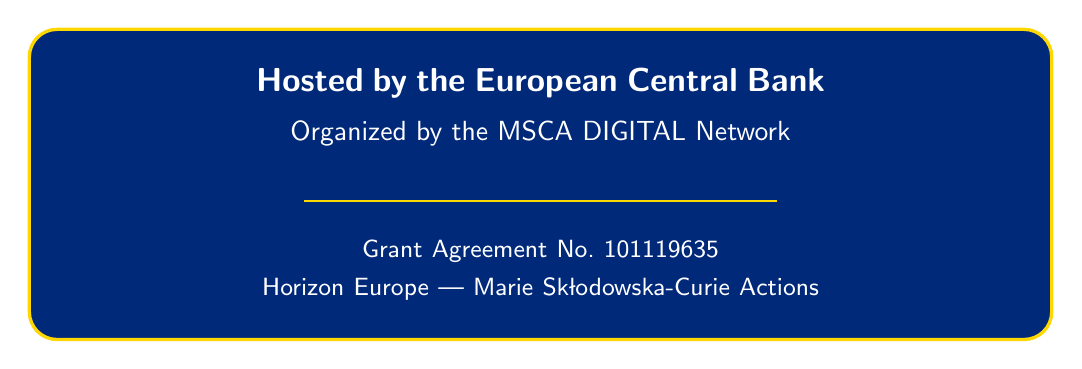
\begin{tikzpicture}
    \node[draw=confgold, rounded corners=10pt, line width=1.2pt,
          inner sep=14pt, text=white, fill=confblue!80!black,
          text width=12cm, align=center] {%
      {\large\bfseries Hosted by the European Central Bank}\\[6pt]
      {\normalsize Organized by the MSCA DIGITAL Network}\\[10pt]
      {\color{confgold}\rule{6cm}{0.5pt}}\\[8pt]
      {\small Grant Agreement No.\ 101119635}\\[2pt]
      {\small Horizon Europe --- Marie Sk\l{}odowska-Curie Actions}
    };
  \end{tikzpicture}
\end{center}

\vfill
\begin{center}
  {\color{white!60}\footnotesize
    Sonnemannstrasse 20 \,$\cdot$\, 60314 Frankfurt am Main \,$\cdot$\, Germany}
\end{center}
\vspace{0.5cm}

\clearpage
\nopagecolor

% ============================================================================
% PAGE 2: FOREWORD
% ============================================================================

\sectiontitle{Welcome}

\vspace{2pt}
{\itshape\color{gray}\large A letter from the co-chairs}
\vspace{8pt}

\begin{spacing}{1.15}
\noindent Dear colleagues and friends,

It is our great pleasure to welcome you to the \textbf{Digital Finance for Supervision} workshop, hosted at the \textbf{European Central Bank} in Frankfurt am Main on December~3, 2026. This event brings together ECB supervision experts with researchers from the MSCA DIGITAL network to explore how artificial intelligence, machine learning, and natural language processing are transforming the landscape of banking supervision.

The \textbf{DIGITAL network} --- funded by the European Union's Horizon Europe programme under the Marie Sk\l{}odowska-Curie Actions --- unites 22 partner institutions from across Europe, including universities, central banks, financial institutions, and technology companies. Our shared mission is to advance the frontiers of digital finance research while training the next generation of researchers who can navigate both the technical and regulatory dimensions of financial innovation.

Today's workshop focuses on three interconnected research themes: AI/ML applications for bank supervision, NLP for regulatory reporting, and the emerging role of large language models in supervisory processes. We have assembled a programme featuring keynote addresses, contributed research presentations, and panel discussions designed to bridge the gap between cutting-edge academic research and real-world supervisory practice.

We are particularly grateful to the ECB for hosting this event and for the active engagement of ECB staff in both the organization and the intellectual programme. We encourage you to engage actively in the discussions, connect with fellow researchers and practitioners, and explore opportunities for collaboration.
\end{spacing}

\vspace{16pt}
\begin{center}
\sigblock{Theodoros Mastrokostopoulos}{ECB Lead Organizer}{European Central Bank}
\hfill
\sigblock{Joerg Osterrieder}{DIGITAL Network Coordinator}{University of Twente}
\end{center}

\vfill

% Workshop Themes filler box
\noindent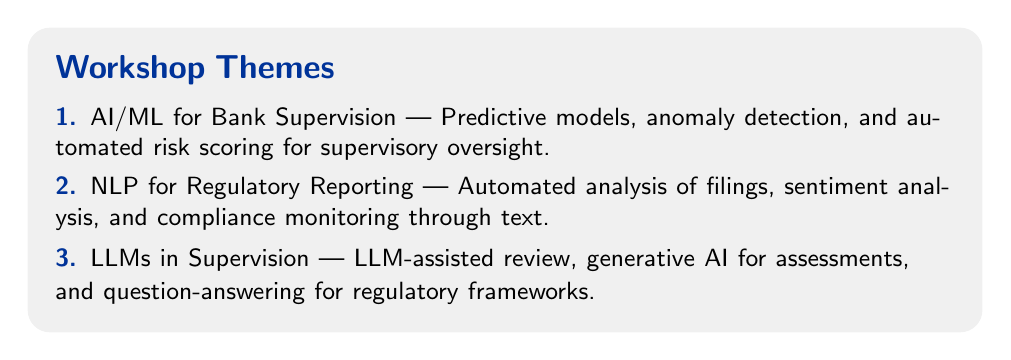
\begin{tikzpicture}
  \node[fill=conflight, rounded corners=8pt,
    text width=\linewidth-20pt, inner sep=10pt, align=left] {%
    {\color{confblue}\bfseries\large Workshop Themes}\\[6pt]
    {\small
    \textbf{\color{confblue}1.} AI/ML for Bank Supervision --- Predictive models, anomaly detection, and automated risk scoring for supervisory oversight.\\[3pt]
    \textbf{\color{confblue}2.} NLP for Regulatory Reporting --- Automated analysis of filings, sentiment analysis, and compliance monitoring through text.\\[3pt]
    \textbf{\color{confblue}3.} LLMs in Supervision --- LLM-assisted review, generative AI for assessments, and question-answering for regulatory frameworks.}
  };
\end{tikzpicture}

\clearpage

% ============================================================================
% PAGE 3: ABOUT + KEY FACTS
% ============================================================================

\sectiontitle{About the Workshop}

\vspace{2pt}
\noindent The \textbf{Digital Finance for Supervision} workshop brings together researchers from the MSCA DIGITAL network and supervision practitioners from the European Central Bank to explore how artificial intelligence, natural language processing, and large language models are reshaping financial supervision across Europe. This half-day event features keynote presentations, research sessions, and panel discussions designed to foster meaningful dialogue between academia and supervisory practice.

\vspace{12pt}

% Stats boxes row
\begin{center}
\statbox{30+}{PARTICIPANTS}
\hspace{6pt}
\statbox{6}{RESEARCH TALKS}
\hspace{6pt}
\goldstatbox{2}{KEYNOTES}
\hspace{6pt}
\statbox{20+}{PARTNER INSTITUTIONS}
\end{center}

\vspace{14pt}

% Important Dates box
\noindent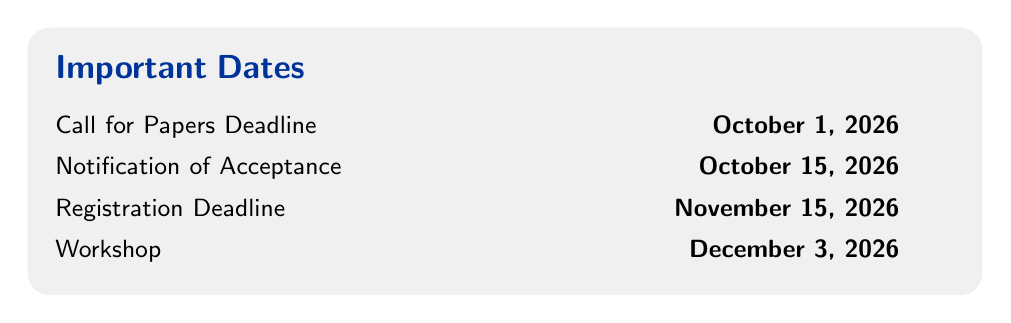
\begin{tikzpicture}
  \node[fill=conflight, rounded corners=8pt,
    text width=\linewidth-20pt, inner sep=10pt, align=left] {%
    {\color{confblue}\bfseries\large Important Dates}\\[8pt]
    \begin{tabularx}{\linewidth-20pt}{@{}X r@{}}
      {\small Call for Papers Deadline} & {\small\bfseries October 1, 2026}\\[3pt]
      {\small Notification of Acceptance} & {\small\bfseries October 15, 2026}\\[3pt]
      {\small Registration Deadline} & {\small\bfseries November 15, 2026}\\[3pt]
      {\small Workshop} & {\small\bfseries December 3, 2026}\\
    \end{tabularx}
  };
\end{tikzpicture}

\vspace{12pt}

% QR code
\begin{center}
  \qrcode[height=2.5cm]{https://digital-ai-finance.github.io/digital-finance-supervision/}\\[6pt]
  \styledurl{https://digital-ai-finance.github.io/digital-finance-supervision/}
\end{center}

\vspace{10pt}

% Who Should Attend? filler box
\noindent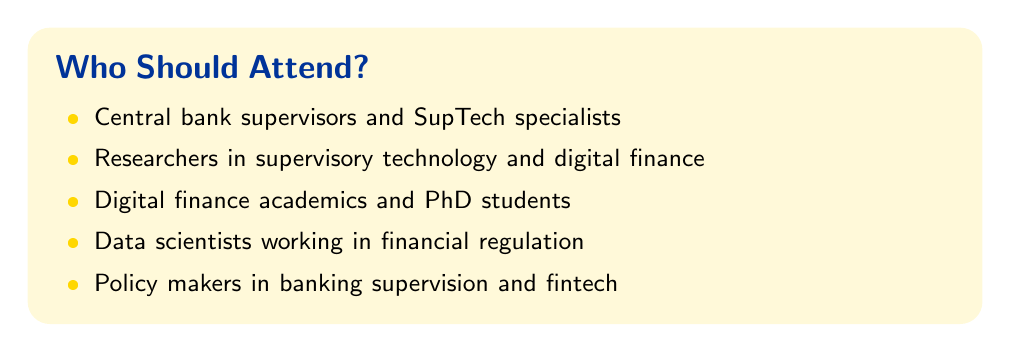
\begin{tikzpicture}
  \node[fill=confgold!15, rounded corners=8pt,
    text width=\linewidth-20pt, inner sep=10pt, align=left] {%
    {\color{confblue}\bfseries\large Who Should Attend?}\\[6pt]
    {\small
    \begin{itemize}[leftmargin=14pt, itemsep=2pt, label={\color{confgold}\textbullet}]
      \item Central bank supervisors and SupTech specialists
      \item Researchers in supervisory technology and digital finance
      \item Digital finance academics and PhD students
      \item Data scientists working in financial regulation
      \item Policy makers in banking supervision and fintech
    \end{itemize}}
  };
\end{tikzpicture}

\vfill
{\centering\small\color{gray} Registration is free of charge --- funded by the MSCA DIGITAL Network (GA 101119635).\par}

\clearpage

% ============================================================================
% PAGE 4: PROGRAM AT A GLANCE
% ============================================================================

\sectiontitle{Program at a Glance}

\vspace{4pt}

% Day header
\noindent
\begin{tikzpicture}
  \node[fill=confblue, rounded corners=6pt,
    text width=\linewidth-16pt, inner sep=8pt, align=center]
    {{\large\bfseries\color{white} Thursday, December 3, 2026}};
\end{tikzpicture}

\vspace{8pt}

\renewcommand{\arraystretch}{1.5}
\noindent\begin{tabularx}{\textwidth}{@{}>{\raggedright}p{2.8cm} X@{}}
\toprule
\progtime{10:00} & \progbreak{Registration \& Welcome Coffee}\\
\progtime{10:15} & \progsession{Opening Remarks} --- Welcome by ECB and DIGITAL Network representatives\\
\rowcolor{confgold!12}
\progtime{10:30} & \progsession{Keynote 1} --- Invited keynote on AI/ML in bank supervision (Speaker TBA)\\
\progtime{11:15} & \progsession{Research Session 1: AI/ML for Bank Supervision}\\
& {\small\color{confdark} 11:15 -- Research Talk 1 \,$\cdot$\, 11:30 -- Research Talk 2 \,$\cdot$\, 11:45 -- Research Talk 3}\\
\rowcolor{confgray!50}
\progtime{12:00} & \progbreak{Lunch Break \& Networking}\\
\rowcolor{confgold!12}
\progtime{13:00} & \progsession{Keynote 2 / Panel: LLMs in Supervision} (Speaker TBA)\\
\progtime{13:45} & \progsession{Research Session 2: NLP \& SupTech Applications}\\
& {\small\color{confdark} 13:45 -- Research Talk 4 \,$\cdot$\, 14:00 -- Research Talk 5 \,$\cdot$\, 14:15 -- Research Talk 6}\\
\rowcolor{confgold!12}
\progtime{14:30} & \progsession{Panel Discussion: The Future of Digital Supervision}\\
& {\small\color{confdark} Moderated discussion with ECB experts and network researchers}\\
\progtime{14:50} & \progsession{Closing Remarks} --- Summary and outlook by workshop co-chairs\\
\bottomrule
\end{tabularx}
\renewcommand{\arraystretch}{1.0}

\vspace{12pt}

% Session format info box
\noindent
\begin{tikzpicture}
  \node[fill=conflight, rounded corners=6pt,
    text width=\linewidth-16pt, inner sep=8pt, align=left] {%
    {\color{confblue}\bfseries Session Format}\\[4pt]
    {\small Each research session features 3 presentations of 15 minutes each. Speakers and titles will be confirmed after the call-for-papers review process. Submissions are welcome on all three workshop themes.}
  };
\end{tikzpicture}

\vfill

% Networking Opportunities filler box
\noindent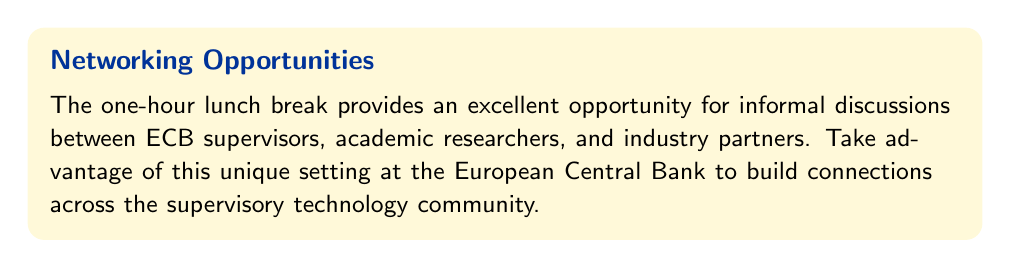
\begin{tikzpicture}
  \node[fill=confgold!15, rounded corners=6pt,
    text width=\linewidth-16pt, inner sep=8pt, align=left] {%
    {\color{confblue}\bfseries Networking Opportunities}\\[4pt]
    {\small The one-hour lunch break provides an excellent opportunity for informal discussions between ECB supervisors, academic researchers, and industry partners. Take advantage of this unique setting at the European Central Bank to build connections across the supervisory technology community.}
  };
\end{tikzpicture}

\clearpage

% ============================================================================
% PAGE 5: ORGANIZING COMMITTEE
% ============================================================================

\sectiontitle{Organizing Committee}

\vspace{4pt}

% Co-Chairs subsection
{\large\bfseries\color{confblue} Co-Chairs}\par\vspace{2pt}
{\color{confgold}\rule{4cm}{1.5pt}}\par\vspace{8pt}

\noindent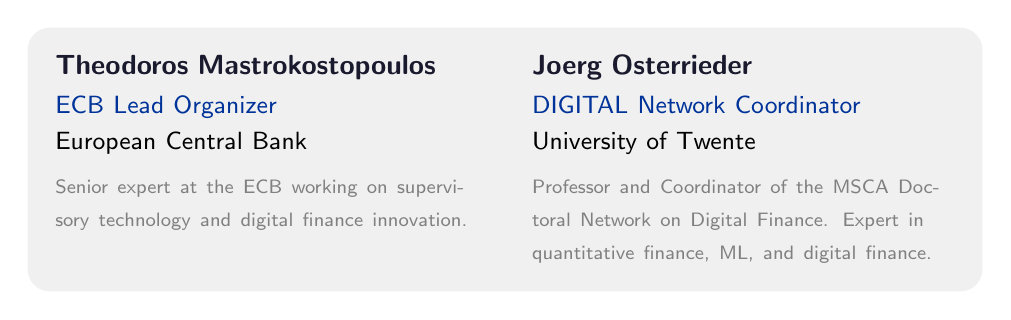
\begin{tikzpicture}
  \node[fill=conflight, rounded corners=8pt,
    text width=\linewidth-20pt, inner sep=10pt, align=left] {%
    \begin{minipage}[t]{0.47\linewidth}
      {\bfseries\color{confdark} Theodoros Mastrokostopoulos}\\[2pt]
      {\small\color{confblue} ECB Lead Organizer}\\[1pt]
      {\small European Central Bank}\\[4pt]
      {\scriptsize\color{gray} Senior expert at the ECB working on supervisory technology and digital finance innovation.}
    \end{minipage}
    \hfill
    \begin{minipage}[t]{0.47\linewidth}
      {\bfseries\color{confdark} Joerg Osterrieder}\\[2pt]
      {\small\color{confblue} DIGITAL Network Coordinator}\\[1pt]
      {\small University of Twente}\\[4pt]
      {\scriptsize\color{gray} Professor and Coordinator of the MSCA Doctoral Network on Digital Finance. Expert in quantitative finance, ML, and digital finance.}
    \end{minipage}
  };
\end{tikzpicture}

\vspace{14pt}

% Committee member grid
{\large\bfseries\color{confblue} Committee Members}\par\vspace{2pt}
{\color{confgold}\rule{4cm}{1.5pt}}\par\vspace{10pt}

% Row 1
\noindent\hfill
\memberblock{TM}{Theodoros Mastrokostopoulos}{European Central Bank}
\hfill
\memberblock{FB}{Filippo Bartoli}{European Central Bank}
\hfill
\memberblock{JO}{Joerg Osterrieder}{University of Twente}
\hfill\null

\vspace{12pt}

% Row 2
\noindent\hfill
\memberblock{DP}{Daniel Pele}{ASE Bucharest}
\hfill
\memberblock{WH}{Wolfgang Haerdle}{HU Berlin / WU Wien}
\hfill
\memberblock{MI}{Maria Iannario}{University of Naples Federico II}
\hfill\null

\vspace{12pt}

% Row 3
\noindent\hfill
\memberblock{CM}{Codruta Mare}{Babes-Bolyai University}
\hfill
\memberblock{CT}{Claudia Tarantola}{University of Milan}
\hfill
\memberblock{AT}{Alessandra Tanda}{University of Pavia}
\hfill\null

\vfill

% MSCA DIGITAL network description box
\noindent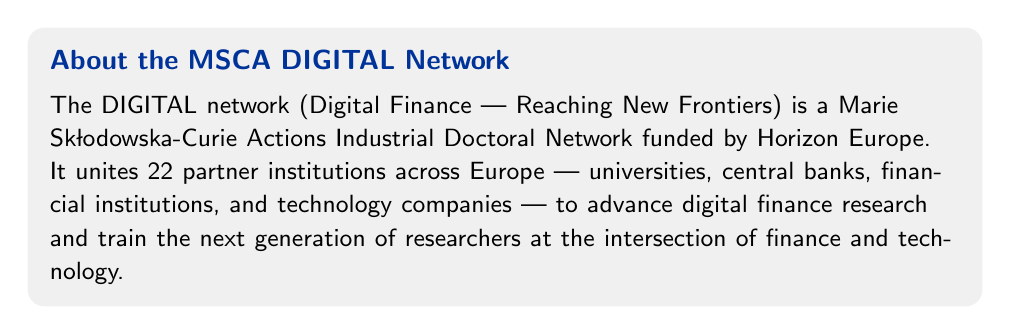
\begin{tikzpicture}
  \node[fill=conflight, rounded corners=6pt,
    text width=\linewidth-16pt, inner sep=8pt, align=left] {%
    {\color{confblue}\bfseries About the MSCA DIGITAL Network}\\[4pt]
    {\small The DIGITAL network (Digital Finance --- Reaching New Frontiers) is a Marie Sk\l{}odowska-Curie Actions Industrial Doctoral Network funded by Horizon Europe. It unites 22 partner institutions across Europe --- universities, central banks, financial institutions, and technology companies --- to advance digital finance research and train the next generation of researchers at the intersection of finance and technology.}
  };
\end{tikzpicture}

\clearpage

% ============================================================================
% PAGE 6: RESEARCH TOPICS
% ============================================================================

\sectiontitle{Research Topics}

\vspace{4pt}
{\color{gray}\small The workshop focuses on three interconnected research themes at the frontier of supervisory technology.}
\vspace{8pt}

\topiccard{1}{AI/ML for Bank Supervision}{%
Application of artificial intelligence and machine learning techniques to enhance banking supervision and regulatory oversight.%
\begin{itemize}[leftmargin=14pt, itemsep=1pt, topsep=4pt, label={\color{confgold}\textbullet}]
  \item Predictive models for identifying risks in supervised entities
  \item Anomaly detection in financial reporting data
  \item Automated risk scoring and early warning systems
  \item Machine learning for stress testing and scenario analysis
  \item AI-driven assessment of bank business models
\end{itemize}%
}

\topiccard{2}{NLP for Regulatory Reporting}{%
Natural language processing applied to regulatory documents, compliance monitoring, and supervisory communication.%
\begin{itemize}[leftmargin=14pt, itemsep=1pt, topsep=4pt, label={\color{confgold}\textbullet}]
  \item Automated analysis of regulatory filings and disclosures
  \item Text mining of supervisory reports and assessments
  \item Sentiment analysis of central bank communications
  \item Information extraction from annual reports and prospectuses
  \item Compliance monitoring through textual analysis
\end{itemize}%
}

\topiccard{3}{LLMs in Supervision}{%
Large language models and generative AI for supervisory processes and regulatory technology.%
\begin{itemize}[leftmargin=14pt, itemsep=1pt, topsep=4pt, label={\color{confgold}\textbullet}]
  \item LLM-assisted review of regulatory documentation
  \item Generative AI for drafting supervisory assessments
  \item Question-answering systems for regulatory frameworks
  \item Summarization of complex financial documents
  \item Ethical considerations and hallucination risks in supervisory AI
\end{itemize}%
}

\vfill

% Gold CTA box
\noindent
\begin{tikzpicture}
  \node[fill=confgold!20, draw=confgold, line width=1pt, rounded corners=8pt,
    text width=\linewidth-24pt, inner sep=12pt, align=center] {%
    {\color{confblue}\bfseries\Large Submit Your Research}\\[6pt]
    {\color{confdark}\normalsize Extended abstracts (max 2 pages) due \textbf{October 1, 2026}}\\[4pt]
    {\small\color{gray} Submit to the organizing committee via the workshop website}
  };
\end{tikzpicture}

\clearpage

% ============================================================================
% PAGE 7: VENUE & PRACTICAL INFORMATION
% ============================================================================

\sectiontitle{Venue \& Practical Information}

\vspace{4pt}

% ECB description box
\noindent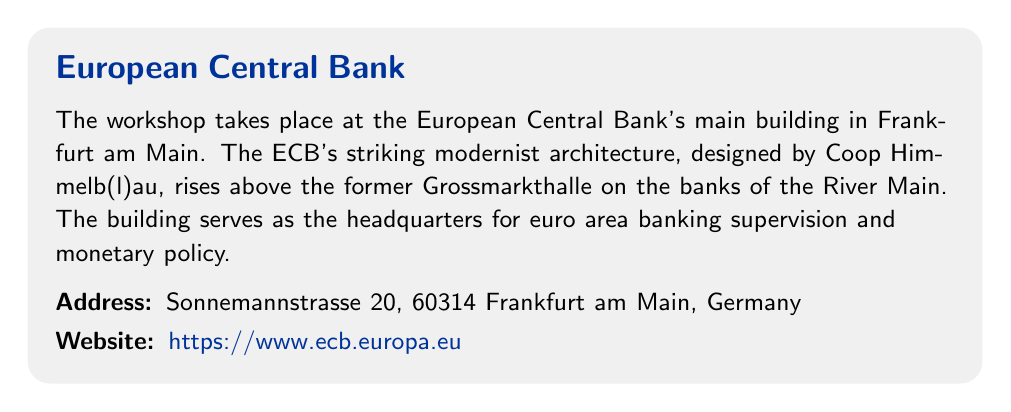
\begin{tikzpicture}
  \node[fill=conflight, rounded corners=8pt,
    text width=\linewidth-20pt, inner sep=10pt, align=left] {%
    {\color{confblue}\bfseries\large European Central Bank}\\[6pt]
    {\small The workshop takes place at the European Central Bank's main building in Frankfurt am Main. The ECB's striking modernist architecture, designed by Coop Himmelb(l)au, rises above the former Grossmarkthalle on the banks of the River Main. The building serves as the headquarters for euro area banking supervision and monetary policy.}\\[6pt]
    {\small\bfseries Address:} {\small Sonnemannstrasse 20, 60314 Frankfurt am Main, Germany}\\[2pt]
    {\small\bfseries Website:} {\small\color{confblue}\url{https://www.ecb.europa.eu}}
  };
\end{tikzpicture}

\vspace{10pt}

% Getting There box
\noindent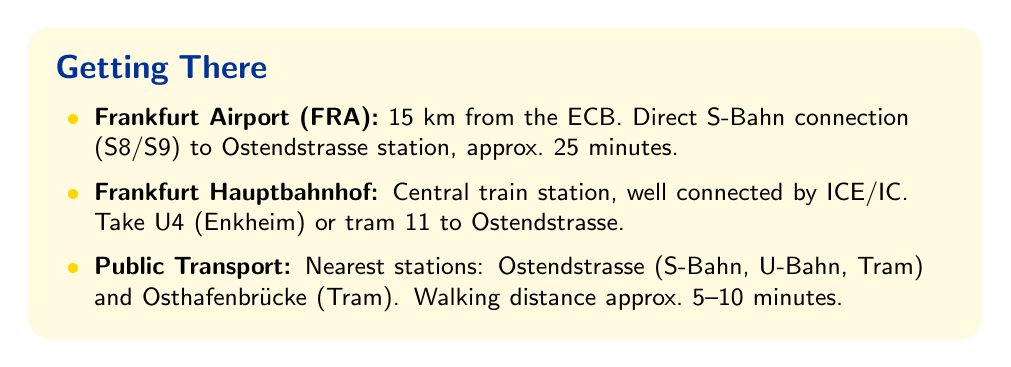
\begin{tikzpicture}
  \node[fill=confgold!12, rounded corners=8pt,
    text width=\linewidth-20pt, inner sep=10pt, align=left] {%
    {\color{confblue}\bfseries\large Getting There}\\[6pt]
    {\small
    \begin{itemize}[leftmargin=14pt, itemsep=3pt, label={\color{confgold}\textbullet}]
      \item \textbf{Frankfurt Airport (FRA):} 15 km from the ECB. Direct S-Bahn connection (S8/S9) to Ostendstrasse station, approx.\ 25 minutes.
      \item \textbf{Frankfurt Hauptbahnhof:} Central train station, well connected by ICE/IC. Take U4 (Enkheim) or tram 11 to Ostendstrasse.
      \item \textbf{Public Transport:} Nearest stations: Ostendstrasse (S-Bahn, U-Bahn, Tram) and Osthafenbr\"ucke (Tram). Walking distance approx.\ 5--10 minutes.
    \end{itemize}}
  };
\end{tikzpicture}

\vspace{10pt}

% Accommodation box
\noindent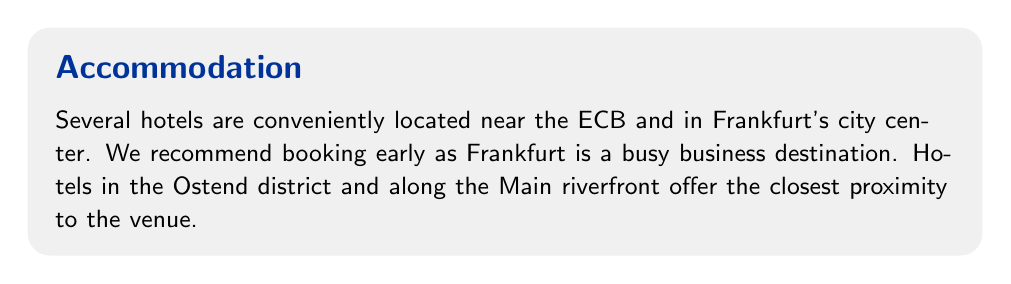
\begin{tikzpicture}
  \node[fill=conflight, rounded corners=8pt,
    text width=\linewidth-20pt, inner sep=10pt, align=left] {%
    {\color{confblue}\bfseries\large Accommodation}\\[6pt]
    {\small Several hotels are conveniently located near the ECB and in Frankfurt's city center. We recommend booking early as Frankfurt is a busy business destination. Hotels in the Ostend district and along the Main riverfront offer the closest proximity to the venue.}
  };
\end{tikzpicture}

\vspace{10pt}

% Practical Details box
\noindent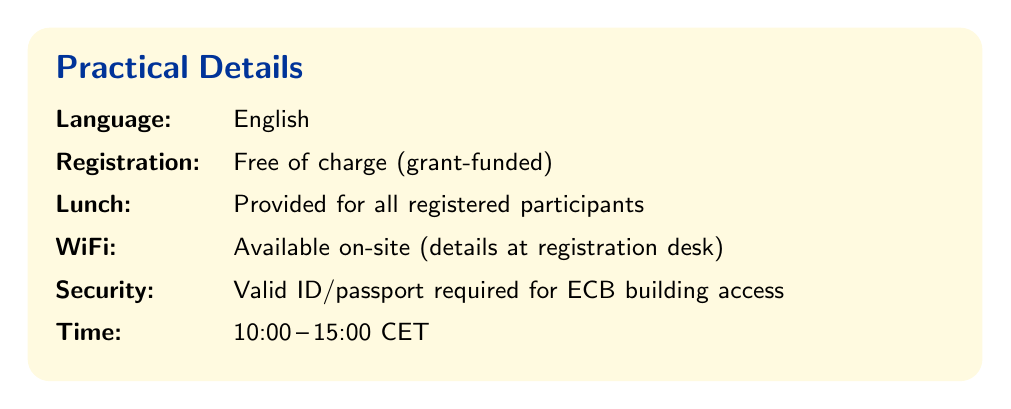
\begin{tikzpicture}
  \node[fill=confgold!12, rounded corners=8pt,
    text width=\linewidth-20pt, inner sep=10pt, align=left] {%
    {\color{confblue}\bfseries\large Practical Details}\\[6pt]
    {\small
    \renewcommand{\arraystretch}{1.4}
    \begin{tabularx}{\linewidth-24pt}{@{}l X@{}}
      \textbf{Language:} & English\\
      \textbf{Registration:} & Free of charge (grant-funded)\\
      \textbf{Lunch:} & Provided for all registered participants\\
      \textbf{WiFi:} & Available on-site (details at registration desk)\\
      \textbf{Security:} & Valid ID/passport required for ECB building access\\
      \textbf{Time:} & 10:00\,--\,15:00 CET\\
    \end{tabularx}
    \renewcommand{\arraystretch}{1.0}}
  };
\end{tikzpicture}

\vfill

\begin{center}
  {\small\color{confblue}\bfseries Contact:} {\small\color{confdark} joerg.osterrieder@utwente.nl}\\[4pt]
  {\scriptsize\color{gray} Please register in advance --- ECB security requires a pre-approved visitor list.}
\end{center}

\clearpage

% ============================================================================
% PAGE 8: PARTNERS & FUNDING
% ============================================================================

\sectiontitle{Partner Institutions}

\vspace{4pt}

% Beneficiary Partners
{\large\bfseries\color{confblue} Beneficiary Partners}\par\vspace{2pt}
{\color{confgold}\rule{4cm}{1.5pt}}\par\vspace{6pt}

\renewcommand{\arraystretch}{1.3}
\noindent\begin{tabularx}{\textwidth}{@{}Xl@{}}
\toprule
\textbf{Institution} & \textbf{Country}\\
\midrule
\rowcolor{conflight}
University of Twente (Coordinator) & Netherlands\\
WU Vienna University of Economics and Business & Austria\\
\rowcolor{conflight}
University of Naples Federico II & Italy\\
Kaunas University of Technology & Lithuania\\
\rowcolor{conflight}
Bucharest University of Economic Studies & Romania\\
Babes-Bolyai University & Romania\\
\rowcolor{conflight}
Cardo AI & Italy\\
Poznan University of Economics and Business & Poland\\
\rowcolor{conflight}
University of Pavia & Italy\\
University of Milan & Italy\\
\rowcolor{conflight}
Bern University of Applied Sciences & Switzerland\\
\bottomrule
\end{tabularx}

\vspace{10pt}

% Associated Partners
{\large\bfseries\color{confblue} Associated Partners}\par\vspace{2pt}
{\color{confgold}\rule{4cm}{1.5pt}}\par\vspace{6pt}

\noindent\begin{tabularx}{\textwidth}{@{}Xl@{}}
\toprule
\textbf{Institution} & \textbf{Country}\\
\midrule
\rowcolor{conflight}
European Central Bank & Germany\\
Deutsche Bank & Germany\\
\rowcolor{conflight}
Raiffeisen Bank International & Austria\\
Swedbank & Lithuania\\
\rowcolor{conflight}
Intesa Sanpaolo & Italy\\
Deloitte & Italy\\
\rowcolor{conflight}
Fraunhofer Institute for Industrial Mathematics & Germany\\
EIT Digital & Belgium\\
\rowcolor{conflight}
Athena Research Centre & Greece\\
Royalton Partners & Luxembourg\\
\rowcolor{conflight}
Bank for International Settlements & Switzerland\\
\bottomrule
\end{tabularx}
\renewcommand{\arraystretch}{1.0}

\vspace{10pt}

% Funding acknowledgment box
\noindent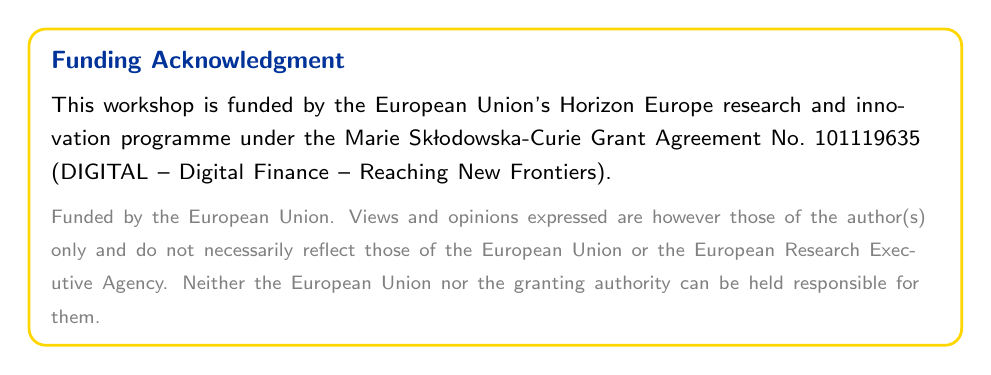
\begin{tikzpicture}
  \node[draw=confgold, line width=1pt, rounded corners=6pt,
    fill=white, text width=\linewidth-24pt, inner sep=8pt, align=left] {%
    {\color{confblue}\bfseries\small Funding Acknowledgment}\\[4pt]
    {\footnotesize This workshop is funded by the European Union's Horizon Europe research and innovation programme under the Marie Sk\l{}odowska-Curie Grant Agreement No.\ 101119635 (DIGITAL -- Digital Finance -- Reaching New Frontiers).}\\[4pt]
    {\scriptsize\color{gray} Funded by the European Union. Views and opinions expressed are however those of the author(s) only and do not necessarily reflect those of the European Union or the European Research Executive Agency. Neither the European Union nor the granting authority can be held responsible for them.}
  };
\end{tikzpicture}

\vfill

% Why Attend? gold-tinted filler box
\noindent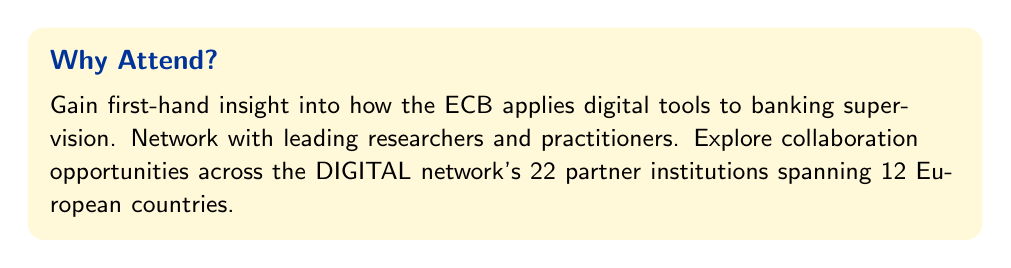
\begin{tikzpicture}
  \node[fill=confgold!15, rounded corners=6pt,
    text width=\linewidth-16pt, inner sep=8pt, align=left] {%
    {\color{confblue}\bfseries Why Attend?}\\[4pt]
    {\small Gain first-hand insight into how the ECB applies digital tools to banking supervision. Network with leading researchers and practitioners. Explore collaboration opportunities across the DIGITAL network's 22 partner institutions spanning 12 European countries.}
  };
\end{tikzpicture}

\clearpage

% ============================================================================
% PAGE 9: BACK COVER
% ============================================================================
\thispagestyle{empty}
\pagecolor{confblue}

\begin{tikzpicture}[remember picture, overlay]
  % Subtle background pattern
  \foreach \i in {1,...,12}{
    \draw[white, opacity=0.03, line width=0.4pt]
      ($(current page.south west) + (\i*1.7, 0)$) -- ++(2,29.7);
  }
  % Top gold bar
  \fill[confgold] (current page.north west) rectangle ($(current page.north east) + (0,-3pt)$);
  % Bottom gold bar
  \fill[confgold, opacity=0.6]
    ($(current page.south west) + (0,1cm)$) rectangle ($(current page.south east) + (0,1.04cm)$);
\end{tikzpicture}

\vspace*{2.5cm}

\begin{center}
  {\fontsize{30}{34}\selectfont\bfseries\color{white}
    Digital Finance\\[6pt] for Supervision}\\[12pt]
  {\color{confgold}\rule{8cm}{1.5pt}}\\[16pt]
  {\Large\color{white} MSCA DIGITAL Network Workshop}\\[6pt]
  {\Large\color{white} European Central Bank}\\[6pt]
  {\large\color{confgold} December 3, 2026}\\[30pt]

  % Large QR code
  
\begin{tikzpicture}
    \node[fill=white, rounded corners=8pt, inner sep=14pt] {%
      \qrcode[height=4cm]{https://digital-ai-finance.github.io/digital-finance-supervision/}
    };
  \end{tikzpicture}\\[14pt]
  {\large\color{white}\bfseries Scan to Visit the Workshop Website}\\[8pt]
  {\color{white}\normalsize\url{https://digital-ai-finance.github.io/digital-finance-supervision/}}\\[30pt]

  {\color{confgold}\rule{6cm}{0.5pt}}\\[12pt]
  {\color{white}\normalsize
    Sonnemannstrasse 20, 60314 Frankfurt am Main, Germany}\\[8pt]
  {\color{white}\normalsize
    Contact: joerg.osterrieder@utwente.nl}\\[8pt]
  {\color{confgold}\normalsize
    December 3, 2026\quad$\cdot$\quad 10:00\,--\,15:00 CET}\\
\end{center}

\vfill

\begin{center}
\begin{minipage}{0.85\textwidth}
  \centering
  {\color{confgold}\rule{0.6\textwidth}{0.5pt}}\\[8pt]
  {\footnotesize\color{white!80}
  Funded by the European Union's Horizon Europe programme.\\
  Grant Agreement No.\ 101119635}\\[8pt]
  {\small\color{confgold}\bfseries
  DIGITAL -- Digital Finance -- Reaching New Frontiers}\\[4pt]
  {\footnotesize\color{white!70}
  Horizon Europe \,$\cdot$\, Marie Sk\l{}odowska-Curie Actions}
\end{minipage}
\end{center}
\vspace{0.8cm}

\clearpage

\end{document}
